\section{Security Analysis}
\label{sec:securityAnalysis}

In this section, we analyze the security of \name by modeling the interaction between the user, host and the remote server.


\begin{figure}[t]
\begin{center}
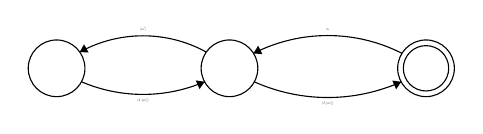
\begin{tikzpicture}[scale=0.15]
\tikzstyle{every node}+=[inner sep=0pt]
\draw [black] (66,-23.1) circle (3);
\draw (66,-23.1) node {\server};
\draw [black] (66,-23.1) circle (2.4);
\draw [black] (45.2,-23.1) circle (3);
\draw (45.2,-23.1) node {\host};
\draw [black] (26.9,-23.1) circle (3);
\draw (26.9,-23.1) node {\user};
\draw [black] (47.743,-21.516) arc (116.95563:63.04437:17.332);
\fill [black] (47.74,-21.52) -- (48.68,-21.6) -- (48.23,-20.71);
\draw (55.6,-19.13) node [above] {$m$};
\draw [black] (29.352,-21.382) arc (118.8302:61.1698:13.89);
\fill [black] (29.35,-21.38) -- (30.29,-21.43) -- (29.81,-20.56);
\draw (36.05,-19.16) node [above] {$[m']$};
\draw [black] (42.565,-24.526) arc (-66.78269:-113.21731:16.527);
\fill [black] (42.57,-24.53) -- (41.63,-24.38) -- (42.03,-25.3);
\draw (36.05,-26.36) node [below] {$(I,[m'])$};
\draw [black] (63.369,-24.535) arc (-65.91058:-114.08942:19.034);
\fill [black] (63.37,-24.53) -- (62.43,-24.4) -- (62.84,-25.32);
\draw (55.6,-26.69) node [below] {$(I,[m'])$};
\end{tikzpicture}
\end{center}
\caption{Finite state machine that depicts the interaction between the user (\user), host (\host) and the server (\server).}
\label{fig:fsm}
\end{figure}

\begin{figure}[t]
\begin{center}
\tikzset{
  every picture/.append style={
    transform shape,
    scale=0.8
  }
 }
\begin{sequencediagram}
\newinst{u}{\user}
\newinst[3]{h}{\host}
\newinst[3]{s}{\server}
\mess{s}{$m$}{h}
\mess{h}{$[m']_1$}{u}
\mess{u}{$I_1,[m']_1$}{h}
%\mess{h}{$[m']_2$}{u}
%\mess{u}{$I_2,[m']_2$}{h}
\mess{h}{...}{u}
\mess{u}{...}{h}
\mess{h}{$[m']_n$}{u}
\mess{u}{$I_n,[m']_n$}{h}
\mess{h}{$I_1,I_2,...,I_n$}{s}
\mess{h}{$[m']_1,[m']_2,...,[m']_n$}{s}
\end{sequencediagram}
\end{center}
\caption{Protocol transcript between the \server, \user and \host that shows one trace from the FSM depicted in Figure~\ref{fig:fsm}.}
\label{fig:protocol}
\end{figure}

\subsection{Modelling the Protocol}
\label{sec:securityAnalysis:modelling}

\subsubsection{Modelling the user behavior}
\label{sec:securityAnalysis:modelling:user}

Correctly understanding the user behaviour is critical as \name focuses to secure user interaction with the remote server. In Section~\ref{sec:systemDesign:userAttention}, we explain secure attention sequence (SAS) (Section~\ref{sec:systemDesign:userAttention:sas}) that \name uses to provide visual cues. SAS enables use to i) follow the legitimate mouse pointer, and ii) recognize which part of the screen is overlaid by the \device. This is achieved by dimming out the screen except the pointer and the UI overlay. We assume that the user behaves reasonably, hence the SAS mechanism is sufficient to isolate the trusted part of the screen (\device overlay) from the untrusted part of the screen. We also agree that system like \name may not achieve absolute security as the user may choose to ignore all visual cues made by the \device and choose to follow the untrusted notification from the host. Therefore, as long as the user does not get influenced by the information provided in the untrusted part of the screen and modifies her input, the \name remains secure.


\subsection{Proof of Integrity}
\label{sec:securityAnalysis:integrity}

From the theorem that are described in Section~\ref{sec:securityAnalysis:modelling}, we can prove that \name provide input integrity. The UI overlay ensures that the user has output integrity, i.e., all the sensitive information sent by the server can not be manipulated by the host. Also the \device signs all the input provided by the user. From Theorem~\ref{theorem:th3}, we can conclude that \name provides IO integrity as long as we assume that the user does not get influenced by any information shown in the non-overlaid part of the screen (Discussed in Section~\ref{sec:securityAnalysis:modelling:user}). \name additionally protects against replay attack as the form also contains nonce to ensure freshness.  

\myparagraph{Attack on the mouse pointer tracking and overlay} The attacker may try to defeat \name mouse pointer tracking and overlay mechanism that is described in Section~\ref{sec:systemDesign:analysis} by introducing a mouse pointer that is visually more detectable by the user. Note that the \device overlaid mouse pointer is quite prominent and hard to miss. One can visualize it as an arms race between the attacker and the \device to grab the attention of the user. But, we can argue that this is a suboptimal strategy for the attacker as both of the pointers will be visible on the screen that can cause suspicion by the user. Hence, we can conclude that executing clickjacking-like attacks are not possible in \name.

\subsection{Proof of Confidentiality}
The host shows a fake form mimicking the overlay of the device. If the user forgets SAS, he sends all information to the host (e.g., payment details, or e-voting), so the confidentiality is lost. However, the integrity should remain, the device signs only data that user has typed.

\myparagraph{Side-channel leakages} Even though, the \device ensures that no mouse, keyboard data reach to the untrusted host when the user executes some operation over the overlaid UI, one can not rule out side-channel leakages. One example could be the amount of time that user user spends or the entry/exit position of the mouse pointer may reveal some information about the input. 

\subsection{Fast-switching}
The attacker can show QR-code, so the device renders the overlay. The host removes QR-code (and the device removes the overlay), then device shows a fake render that mimics the one from the device to show some malicious views. This can be repeated many times.

\subsection{Hover activity}
The attacker wants to learn what button did the user click by tracking the cursor movement. This should be prevented if the device does not send any event to the host when inside the overlay.


\iffalse
\subsection{Protection against phishing attacks}
\subsection{Keyboard Manipulation Attacks and Defenses}
\subsubsection{Change user selected values}


\subsection{Mouse Manipulation Attacks and Defenses}
\subsubsection{Changing mouse position}
Changing the mouse position can be detected by the device as the device expects to find it in the location that the user provides. 
\subsubsection{Removing the mouse completely}
This is detectable by the \device as the \device no longer finds the mouse pointer in the screen at the designated position.  
\subsubsection{Add mouse cursor to confuse users}

\subsection{UI Manipulation Attacks and Defenses}
\subsubsection{Manipulate the position of the UI elements on the screen}
\fi